\documentclass{article}

% Set page size and margins
\usepackage[a4paper,top=2cm,bottom=2cm,left=3cm,right=3cm,marginparwidth=1.75cm]{geometry}

\usepackage[english]{babel}
\usepackage{enumitem}
\usepackage{doi}
\usepackage{amsmath}
\usepackage{graphicx}
\usepackage{verbatim}
\usepackage{hyperref}

\newcommand{\compresslist}{ % Define a command to reduce spacing within itemize/enumerate environments, this is used right after \begin{itemize} or \begin{enumerate}
	\setlength{\itemsep}{1pt}
	\setlength{\parskip}{0pt}
	\setlength{\parsep}{0pt}
}

\title{MALIS Project Final Deliverable\\.\\Machine Learning\\for\\Autism Spectrum Disorder Diagnosis}

\author{
Giulia Lorini\\
Gaganjot Shan\\
Dario Ferrero\\
}



\begin{document}
\maketitle

\section{Introduction}

\textbf{Autism Spectrum Disorder (ASD)} is a range of neurodevelopmental disorders including classical autism, Asperger syndrome, and pervasive developmental disorder not otherwise specified (PDD-NOS), characterized by impaired social skills, repetitive behaviors, sensory issues, and language delay. More than 1\% of the population falls into this spectrum, with a high imbalance between the sexes, males being 4 to 5 times more likely to be affected than females\cite{defautism}.\\

The high heterogeneity of ASD makes it hard to define diagnostic criteria that can be applied to identify affected children as soon as possible to select optimal treatments. Currently, ASD diagnosis involves long processes and multiple specialists’ evaluations, using behavioural assessment instruments. Application of Machine Learning methods to identify the underlying brain mechanisms could significantly speed up the diagnostic process.\cite{defautism}\cite{abide}\\

Following exploration of the current state of ASD diagnosis current state, we decided to
focus on ASD Diagnosis for female patients, since we agreed that the current disproportion in
the existing male-to-female brain image data necessarily leads to biased predictions against the
minority side: focusing on this open problem, although not expecting to make any breakthrough,
we hope to acquire new insights and aim at thinking of ways to improve our initial performances.


\section{Related Work}

\begin{comment}
\begin{itemize}
\item \textbf{Promises, Pitfalls, Guidelines}\cite{guidelinesml}
\subitem - ABIDEI, corr-matrixes, predictions
\subitem - Same: Approach in feature selection
\subitem - Different: ABIDEII, pre-processing not on our own (CPAC), balance between M/F
\end{itemize}
\end{comment}

The main reference we followed in our work has been a research article offering a comprehensive guide to applying Machine Learning Classifiers on Psychiatric Imaging Data \cite{guidelinesml}. Our decision to base ourselves on this previous study came from the fact that data belonging to the same project we identified (ABIDE \cite{abide}) had been used: by adopting ASD as a case of psychiatric disorder we were able to observe techniques, results and considerations of an early attempt to similar type of work.\\

While the overall structure of our project matches the one portrayed in this paper, we decided to adapt some changes in our strategy towards obtaining the final results. The main difference in our approach has been to utilize the ABIDE-II dataset \cite{abide2}, opting for a higher quality one instead of the former, albeit pre-processed. Having data with which we could equally represent male and female subjects was a priority for our task, not achievable by using the previous version of the dataset, from which the researchers working on \cite{guidelinesml} decided to drop altogether all female subjects.\\

Deciding to adopt the ABIDE-II dataset required us to apply some pre-processing steps to the fMRI data for Feature Extraction: while our goal remained to reach the same type of features utilized in the paper, instead of implementing these steps on our own we reputed best to utilize a popular pre-processing pipeline (CPAC \cite{cpac}), the same that was used to obtain the preprocessed ABIDE-I\cite{preprocabide}.




\section{Dataset and Features}

For the purposes of this project we based our initial data on Brain Images, in particular on \textbf{resting-state functional Magnetic Resonance Imaging data (rs-fMRI)}. Looking for data representative of subjects diagnosed with ASD we found a open source data in the \textbf{Autism Brain Imaging Data Exchange (ABIDE)} project \cite{abide}, offering scans generated over several international sites, but aggregated consistently with open science principles, thus providing two collections amounting to respective sample sizes of 1112 and 1114 subjects. We already mentioned in the previous section why we have favored the most recent collection, ABIDE-II, over the other.\\

Together with the imaging data, comprised of mainly Anatomical MRI and rs-fMRI scans, extensive information is made available both on the image acquisition procedures that took place, and on the phenotypic information of the subjects of the studies. From the latter we were able to obtain most importantly the classification labels (the Diagnostic Group, either "Autism" or "Control"), as well as information on each subject such as age, sex, handedness, and mostly results of other diagnostic tests that were deemed possibly related to an ASD diagnosis. Following the steps in \cite{guidelinesml}, we agreed to use this data to initially filter out possible outliers, identified as individuals having more than 40 years of age or IQ lower than 80. Furthermore, since our main objective has been to study a context with balanced Females and Males subjects, we kept all of the F female samples satisfied the age and IQ constraints (being a significant minority with a F:M ratio of about 1:3) and conserved the same amount of individuals from the opposite sex, making sure that the balance between diagnosed and control individuals remained equal as well. Taking into consideration this initial filtering of the data samples, we began working on the fMRIs 416 subjects, with the following composition:
\begin{itemize}\compresslist
	\item Females autistic: 61
	\item Males autistic: 139
	\item Females control: 156
	\item Males control: 60
	\item Total females: 217
	\item Total males: 199
\end{itemize}



The following steps in preparing our data have been \textbf{image pre-processing} and \textbf{feature extraction}. fMRI images are 4D matrices representing the intensities of 3D pixels (voxels) over a certain time frame: several operations were needed to adapt the original files, from simple reshaping to noise reduction and motion correction. Since we agreed that this step required a decent amount of domain knowledge, in order to complete it properly we opted to utilize existing software: after an initial attempt with \textbf{fmriprep}\cite{fmriprep}, we found an appropriate solution in the \textbf{Configurable Pipeline for the Analysis of Connectomes (CPAC)}\cite{cpac}. By applying the default pipeline on our samples, which took much of our time and (limited) computational resources, we were able not only to obtain the actual pre-processed images, but to extract analytical data on these, such as timeseries analyses and especially correlation matrices between \textbf{Regions Of Interest (ROIs)} in the brain (identified from several atlases).\\

Once again we decided to adapt our work to \cite{guidelinesml}, selecting our feature set out of the 200x200 connectivity matrix based the Craddock atlas. From this symmetrical representation of the relationship between ROIs, a total of 19900 features was selected for each sample.\\

\begin{figure}[h]
	\centering
	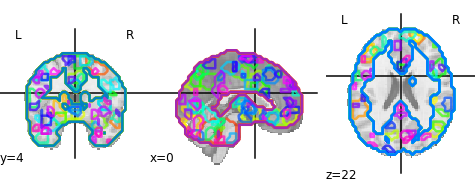
\includegraphics[width=0.75\textwidth]{atlas.png}
	\caption{ROIs highlighted on Craddock atlas}
\end{figure}

In addition, we also repeated the steps that were supposedly taken by C-PAC in the generation of the correlation matrices (we can only guess as to how they were actually obtained due to the lack of in depth documentation) to obtain the correlation matrices for all the processed fMRIs, since we realized that the C-PAC preprocessing script had at times failed to generate the ROI analysis output for some subjects. We followed the general indications of Kassraian-Fard et al.\cite{guidelinesml}, as usual. We downloaded the Craddock atlas from nilearn's\cite{neuroml} database: this atlas is not the same as the one used by C-PAC, because it's a 4D atlas instead of 3D, and it has 120 instead of 200 ROIs. For all those 120 ROIs, we compute the average time series and then the correlation matrix containing the correlation of each pair of time series. The result is a 120x120 symmetric matrix, which translates to 7140 unique features, far less than the ones previous ones. Finally, we applied Fisher's z-transform to the matrix, again as suggested in the paper, to go from a correlation to a connectivity matrix.




\section{Methods}

\paragraph{Logistic Regression}

Logistic Regression is a classification algorithm, which means that it allows to predict the class that an input variable belongs to. In our case there are only two classes (Autistic and Control), so our task is binary classification. It's a linear model, therefore it will try to divide the feature space into two regions, each one corresponding to one of the two classes. The training process for this defines the weight values to be assigned to each of the features involved, depending on how much they're influent in determining the right class. As a measure of estimation for the weight parameters, typically the Cross-Entropy Loss Function is adopted:
$$
\hat{w}_0, \hat{w} = arg_w min -\sum_{i=1}^{N} y_i log\sigma(w_0 + w^T x_i) +
(1 - y_i)log(1-\sigma(w_0 + w^T x_i))
$$

\paragraph{Lasso Regularizer (L1)}

In the context of a Logistic Regression model too much sensitive to new data we might find ourselves having weight values noticeably large. Lasso Regularization, when applied to Logistic Regression, operates by adding a penalty equal to the absolute value of the weights' magnitude. This method for semplification of the model works by calculating a Regularizer function
$$
R(w) = \sum_{i=1}^{D} |w_i|
$$
and applying it to the previously mentioned loss function, which is now updated like this
$$
L(w) + \lambda R(w)
$$
As a hyperparameter, $\lambda \ge 0$ controls the strength of the L1 penalty.  When $\lambda$ = 0, the regularization is not applied at all, whereas for an increasing value we will have an increasingly simple model, with the original weights playing a less relevant role in prediction (and potentially being eliminated).


\paragraph{SVM}

Like Logistic Regression, Support Vector Machines' main goal is to find the best separating hyperplane dividing a dataset in two regions, depending on the data's labels. Their peculiarity lies in attempting to find not any hyperplane, but the one maximizing the distance between the closest data points belonging to different classes (Support Vectors). Depending on whether a model allows a data point to fall into the opposite side of the hyperplane or not, an SVM is called soft- or hard-margin.

\begin{figure}[h]
	\centering
	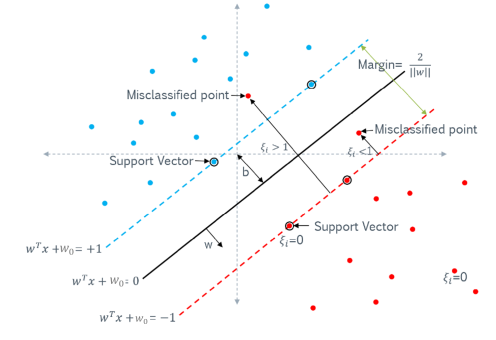
\includegraphics{svm}
	\caption{An example of soft-margin SVM}
\end{figure}


\paragraph{(k-Fold) Cross Validation}

This technique is used for evaluating a model when facing limited samples of data. The basic idea is to subdivide the whole dataset in $k$ partitions (folds): for $k$ iterations, a different partition is used as testing set, while the remaining $k-1$ as training data for the k-th model.
The average of the $k$ testing accuracies gives us in this case a better performance measurement if compared to a simple train/test split.\\
We combined 5-fold stratified cross validation with grid search for hyperparameter tuning, using a nested cross validation approach to automatically choose and work on the best model. In the outer loop of our nested cross validation we used repeated (10 iterations) stratified 5-fold cross validation, and simple stratified 5-fold CV in the inner loop. Repeating the k-fold cross validation process is useful to have a better estimate of the model's performance by trying different splits of the dataset and reporting the mean performance found\cite{repeated_kfold}.

\paragraph{Grid Search}

Grid Search is a method used to systematically look for the best hyperparameters for a model, by performing a complete grid search based on some provided parameters.

\section{Experiments}

\begin{comment}
	\begin{itemize}
	\item Cross-validation, folds, etc.
	\item Metrics used: accuracy, precision, AUC...
	\item Both quantitative and qualitative results
	\item Add some kind of image / plot
	\item Overfitting?
	\end{itemize}
\end{comment}

With our dataset formed by the features and labels obtained as described in the previous sections, we attempted to train two different classifiers: a Logistic Regression with L1 Regularization, and a Support Vector Machine Linear Classifier. Validation and testing were introduced by implementing Nested k-fold Cross Validation, as explained in the previous section. We used a "Repeated 5-fold Cross Validation" as an alternative to increasing the 'k' number of splits, which we can't afford to do with the size of our dataset otherwise our splits would become too small. We chose the "stratified" version so that our splits would maintain the 1:1 ratio of autistic and control subjects, and we set "shuffle" to True to select the samples randomly when forming the split sets, which we considered important because our data was ordered by subject id, which means that it was basically grouped by testing site. By shuffling we hope to remove any bias in the data related to conditions specific to the fMRI machine used, that may still be present even after all the image processing steps. A Grid Search was used to find the optimal regularization strength ("C" parameter), and the model is refit at each iteration of the nested k-fold CV using the best result. \\
We tried both with the correlation matrices and the connectivity matrices as features, but we couldn't see significant differences between the two.

The results are, as expected, not great: the best performance is given by the SVM model with C=0.013, with a testing accuracy of 0.573, slightly higher than a dummy classifier obtained with "stratified" strategy, which in particularly lucky runs can score around 0.55. As bad as this looks, the result is in line with what was reported in our reference paper \cite{guidelinesml}, who had 0.58 for that same classifier. We were in fact expecting to have a slightly worse performace than theirs, on account of their choice to remove female subjects from their input data because of the known strong differences in the female neuropathology of autism, and as a consequence of that, they also had a bigger input dataset to work with because they didn't have to cut it to keep the sex balance.
We observed that, in general, both models appear to easily overfit over the data, reaching very easily an average training accuracy close to 100\% even with tiny changes of the regularization parameter C.\\

Since our objective was to provide a model that would diagnose with some amount of precision even female subjects (or at least with better accuracy than models trained on exclusively male data as are all that we're aware of) we tested the final model with a previously set aside (not used in the steps described above) subset of only females and then with only males, to check gender-specific performance. We could see that indeed with some models the performance is surprisingly good, even if with huge variations (between 0.4 and 0.7). That could also be due to the small sample that we're testing upon, so with more time we could run more (and better) tests to get a better idea of the true performance.
\begin{figure}[h]
	\centering
	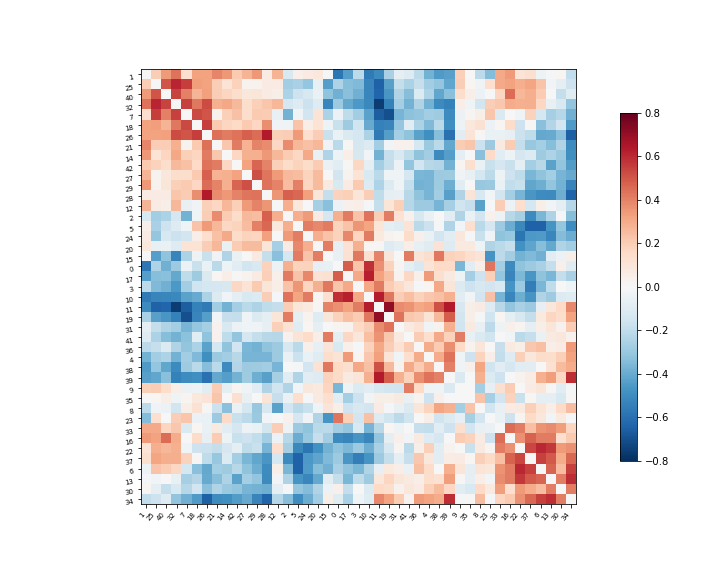
\includegraphics{img/corr_matrix}
	\caption{An example of soft-margin SVM}
\end{figure}


\section{Conclusions}
\begin{comment}
	\textit{For	future work, if you had more time, more team members, or more computational resources, what would you explore?}
\end{comment}

As ASD diagnosis via Machine Learning remains an open problem, much is still to be done from a research point of view as well as experimentations we would have liked to try. Much depends on the type and quantity of data that will be collected in the future regarding female ASD neuropathology, which would help with creating a model specific or that category. With more computational resources (and time) we would have liked to continue trying with the entire fMRI data as features, instead of performing dimensionality and feature reduction to move to the correlation and connectivity matrices.
It would also be interesting to try other classifiers, both linear and non-linear.

\section{Contributions}
\begin{itemize}
	\item \textbf{Common:} Data collection and project planning.
	\item \textbf{Giulia Lorini:} Project management, main research analysis, baseline code preparation, data selection and pre-processing, brain image manipulation and feature extraction.
	\item \textbf{Dario Ferrero:} Data wrangling, pre-processing configuration, debugging, baseline training, report composition.
	\item \textbf{Gaganjot Shan:} Dataset analysis, papers analysis, attempt to fit a model with ABIDEII Composite Phenotype and Phenotype V10b (tabular) data as input.
\end{itemize}

\clearpage
% !TEX encoding = IsoLatin
\begin{thebibliography}{9}
\addcontentsline{toc}{section}{Riferimenti bibliografici}

\bibitem{defautism}
Gene Blatt,
``autism'',
Encyclopedia Britannica,
9 Sep. 2021,
\url{https://www.britannica.com/science/autism},
Accessed 27 October 2021.

\bibitem{abide}
Child Mind Institute,
``Autism Brain Imaging Data Exchange'',
ABIDE,
Child Mind Institute,
\url{http://fcon_1000.projects.nitrc.org/indi/abide/},
Accessed 27 October 2021.

\bibitem{sexdiff}
Kaat Alaerts, Stephan P. Swinnen, and Nicole Wenderoth.,
``Sex Differences in Autism: A Resting-State Fmri Investigation of Functional Brain Connectivity in Males and Females.'',
Social cognitive and affective neuroscience.,
U.S. National Library of Medicine.,
Accessed October 27, 2021.,
\url{https://pubmed.ncbi.nlm.nih.gov/26989195/}.

\bibitem{preprocabide}
Cameron Craddock, Pierre Bellec.,
``ABIDE Preprocessed.'',
Preprocessed Connectomes Project.,
Accessed October 27, 2021.,
\url{http://preprocessed-connectomes-project.org/abide/}.

\bibitem{neuroimg}
Cameron Craddock, Yassine Benhajali, Carlton Chu, Francois Chouinard, Alan Evans, András Jakab, Budhachandra Singh Khundrakpam, John David Lewis, Qingyang Li, Michael Milham, Chaogan Yan, Pierre Bellec,
``The Neuro Bureau Preprocessing Initiative: open sharing of preprocessed neuroimaging data and derivatives.'',
In Neuroinformatics 2013,
Stockholm, Sweden,
\doi{10.3389/conf.fninf.2013.09.00041}.

\bibitem{abide2}
Child Mind Institute.,
``Autism Brain Imaging Data Exchange II'',
ABIDE. Child Mind Institute., \url{http://fcon_1000.projects.nitrc.org/indi/abide/abide_II.html}.,
Accessed 27 October 2021.

\bibitem{guidelinesml}
Pegah Kassraian-Fard, Caroline Matthis, Joshua H. Balsters, Marloes H. Maathuis, Nicole Wenderoth,
``Promises, Pitfalls, and Basic Guidelines for Applying Machine Learning Classifiers to Psychiatric Imaging Data, with Autism as an Example'',
Frontiers in Psychiatry,
vol. 7,
2016,
ISSN-1664-0640,
\doi{10.3389/fpsyt.2016.00177}

\bibitem{neuroml}
Abraham, Alexandre and Pedregosa, Fabian and Eickenberg, Michael and Gervais, Philippe and Mueller, Andreas and Kossaifi, Jean and Gramfort, Alexandre and Thirion, Bertrand and Varoquaux, Gael,
``Machine learning for neuroimaging with scikit-learn'',
Frontiers in Neuroinformatics,
vol. 8,
2014,	
\url{https://www.frontiersin.org/article/10.3389/fninf.2014.00014},
ISSN 1662-5196,
Statistical machine learning methods are increasingly used for neuroimaging data analysis. Their main virtue is their ability to model high-dimensional datasets, e.g., multivariate analysis of activation images or resting-state time series. Supervised learning is typically used in decoding or encoding settings to relate brain images to behavioral or clinical observations, while unsupervised learning can uncover hidden structures in sets of images (e.g., resting state functional MRI) or find sub-populations in large cohorts. By considering different functional neuroimaging applications, we illustrate how scikit-learn, a Python machine learning library, can be used to perform some key analysis steps. Scikit-learn contains a very large set of statistical learning algorithms, both supervised and unsupervised, and its application to neuroimaging data provides a versatile tool to study the brain,
\doi{10.3389/fninf.2014.00014}

\bibitem{fmriprep}
``fMRIPrep: A Robust Preprocessing Pipeline for fMRI Data'',
\url{https://fmriprep.org/en/stable/}

\bibitem{andysbrainbook}
\url{https://andysbrainbook.readthedocs.io/}

\bibitem{cpac}
``Configurable Pipeline for the Analysis of Connectomes (C-PAC)'',
\url{https://fcp-indi.github.io/}

\bibitem{repeated_kfold}
    ``Repeated k-fold Cross Validation with python'',
    \url{https://machinelearningmastery.com/repeated-k-fold-cross-validation-with-python/}


\end{thebibliography}


\end{document}
